\documentclass{beamer}
\usetheme{Darmstadt}
\usecolortheme{beaver}
\usepackage{booktabs}
\usepackage{hyperref}

\usepackage[utf8]{inputenc}
\usepackage{graphicx}
\graphicspath{ {./images/} }

%Information to be included in the title page:
\title{Homework 02}
\author{Brandon Hosley}
\institute{University of Illinois - Springfield}
\date{\today}

\begin{document}
\frame{\titlepage}

\begin{frame}{Overview}
\tableofcontents
\end{frame}

\section[Q1]{Q1: Bias–variance tradeoff}

\begin{frame}{Bias-Variance Trade-Off}
	\begin{columns}
		\column{0.5\textwidth}
		Bias Error
		\begin{itemize}
			\item<1-> Also called 'Overfitting'
			\item<4-> Predicts test data too well
		\end{itemize}
		
		\column{0.5\textwidth}
		Variance 
		\begin{itemize}
			\item<2-> Also called 'Underfitting'
			\item<5-> Generalizes too well
		\end{itemize}
	\end{columns}
	\centering
	\onslide<3->{\includegraphics[width=0.6\linewidth]{OverAndUnderFit}}
\end{frame}

\begin{frame}{Bias-Variance Trade-Off}
	\begin{itemize}%[<+->]
		\item Aiming for the lowest total error typically means finding a "middle-ground"
		\item A common technique for this is determining the minimum \emph{mean squared error.} 
	\end{itemize}
	\begin{align*}
		\text{MSE} &= \left( E\left[\hat{f}(x)\right]-f(x)\right)^2 + E\left[\left(\hat{f}(x) - E\left[\hat{f}(x)\right]\right)^2\right] +
		\sigma^2_e \\
		&= \text{Bias}^2 + \text{Variance} + \text{Irreducible Error}
	\end{align*}
	\centering
	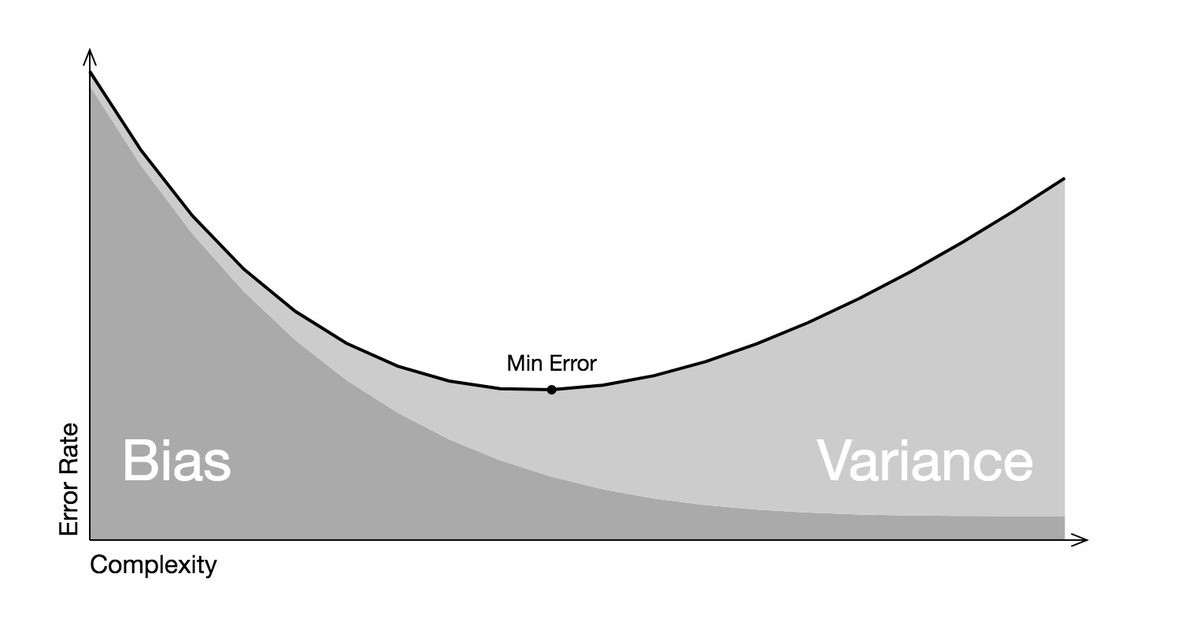
\includegraphics[width=0.5\linewidth]{MinError}
\end{frame}

\section[Q2]{Q2: Hastie and Tibshirani}

\begin{frame}{Hastie Lectures}
	\begin{itemize}
		\item Statistical Learning and Regression
		\item Dimensionality and Parametric Models
		\item Assessing Model Accuracy and Bias-Variance Trade-Off
		\item Classification Problems and K-Nearest Neighbors
	\end{itemize}
\end{frame}

\begin{frame}{Statistical Learning and Regression}
	\begin{itemize}[<+->]
		\item Predicting values through various \emph{means}
		\item The simplest method of regression may be to use: \\ 
			\vspace{0.5em} \hspace{4em} $ \hat{f}(x_n) = \bar{x}_n $
		\item This type of model may be improved by extending the values contributing to the average	to: \\ 
			\vspace{0.5em} \hspace{4em} $ \hat{f}(x_n) = \bar{x}_{n\pm i} $
		\item Or the range may be adjusted such that it includes the $k$-nearest neighbors.
		\item[] \hspace{4em} \includegraphics[width=0.3\linewidth]{NeighborAvg}
	\end{itemize}
\end{frame}

\begin{frame}[t]{Dimensionality and Parametric Models}
	\begin{itemize}[<+->]
		\item Approximate proportion of a data's range needed to capture a certain fraction of the data scales very quickly with added dimensions
		\item[]<only@+> \vspace{0.5em} \hspace{4em}
			\includegraphics[width=0.4\linewidth]{DimensionReqs}
		\item Structured models may help address these scaling problems
		\item[] The simplest structured model is a linear model: \\
			\vspace{0.5em} \hspace{4em} 
			$ f_L(X) = \beta_0 + \beta_1X_1 + \cdots + \beta_nX_n $
		\item Structured models allowed allow flexible adjustment to obtain preferred level of fitting
	\end{itemize}
\end{frame}

\begin{frame}{Assessing Model Accuracy and Bias-Variance Trade-Off}
	\begin{itemize}
		\item<1-> Mean-squared error is a good method for testing accuracy
		\item<3-> But testing against \emph{training} data will bias toward over-fit models
		\item<4-> Measuring against a separate batch of \emph{test} data will likely provide a more accurate model 
		\item[]<1->
		\item[]<only@2-3> \hspace{3em}
			$\text{MSE}_{\text{\textbf{Tr}}}=\text{AVE}_{i\in\text{\textbf{Tr}}}\left[y_i-\hat{f}(x_i)\right]^2$
		\item[]<only@4-> \hspace{3em}
			$\text{MSE}_{\text{\textbf{Te}}}=\text{AVE}_{i\in\text{\textbf{Te}}}\left[y_i-\hat{f}(x_i)\right]^2$
	\end{itemize}
\end{frame}


\begin{frame}{Classification Problems and K-Nearest Neighbors}
	\begin{itemize}[<+->]
		\item Goals:
		\begin{itemize}[<+->]
			\item Build classifier model $\mathcal{C}(X)$
			\item Assess uncertainty of prediction
			\item Understand roles of factors in prediction $X =\left\lbrace X_1, X_2, \ldots, X_n \right\rbrace $
		\end{itemize}
	\end{itemize}
\end{frame}

\section[Q3]{Q3: ISL Section 2.3}
\section[Q4]{Q4: ISL Section 2.4}
%Exercises. No. 10 (p. 56)

\end{document}
